\section{Entwurf elektrischer Maschinen}
\sectionbox{
\subsection{Größen}
\tablebox{
\begin{tabular*}{\columnwidth}{p{4,5cm}cc}
\ctrule
Essonziffer & $C$ & $\unitof{\si{\tesla\ampere\per\meter}}$\\
ideeler Polbogenwinkel & $\beta_{pi}$ & $\unitof{\si{\radian}}$\\
ideele Polbogenlänge & $b_{pi}$ & $\unitof{\si{\meter}}$\\
Rotorstrombelag & $A_2$ & $\unitof{\si{\ampere\per\meter}}$\\
mittlerer Statorstrombelag & $\overline{A}_1$ & $\unitof{\si{\ampere\per\meter}}$\\
relative Länge & $\lambda$ & $\unitof{\si{1}}$\\
Nutfüllfaktor (Stator) & $\kappa_{N1}$ & $\approx\num{0.5}$\\
\cbrule
\end{tabular*}
}

\subsection{Überblick Entwurfsprozess}
\cookbox{Entwurfsprozess}{
\item \textbf{Anforderungsprofil:} meist Nennleistung und Nenndrehzahl
\item \textbf{Grobentwurf:} Hauptabmessungen, Wicklungsschema, Satorentwurf, Rotorentwurf
\item \textbf{Nachrechnung:} Berechnung über analytische Gleichungen (FEM)
\item \textbf{Optimierung:} Anpassung des Grobentwurfs
}
}
\sectionbox{
\subsection{Grobentwurf}
\cookbox{Grobentwurf}{
\item Drehmoment im Nennbetrieb aus $P$ und $n$ bestimmen
\item Ankervolumen über $C$ bestimmen $P_{mi} = C\cdot D_\delta^2l_i\cdot n$
\item Bestimmung des Ankerinnendurchmessers\\
direkt mit $\lambda = \frac{l_i}{\tau_p} = \frac{2p\cdot l_i}{\pi\cdot D_\delta}$\\
indirekt über Ankervolumen
\item Bestimmung des Ankeraußendurchmessers
\item Bestimmung des Wicklungsschemas
\item Statorentwurf
\item Rotorentwurf
}

\subsubsection{Drehmoment}
\emphbox{$M_{D,N} = 2p\cdot\left(\frac{D_\delta}{2}\right)^2\cdot l_i\cdot\int\limits_0^{\frac{\pi}{p}}B_\delta(\vartheta_1,t)\cdot A_2(\vartheta_1,t)\diff\vartheta$}
$\tau_p\cdot\beta_{pi} = b_{pi}$
}
\sectionbox{
\subsubsection{Bestimmung des Innendurchmessers Gleichstrommaschine}
\symbolbox{\begin{center}
$C = \pi^2\beta_{pi}\cdot A_2\cdot B_{\delta,\text{max}}$
\end{center}}
$A_2 = 4w_2\frac{I_A}{2}\frac{1}{\pi D_\delta}$\\
\[D_i = k_1 + k_2\cdot\sqrt[3]{\frac{p\cdot P_{mi}}{\lambda\cdot n}}\quad\text{mit}\begin{cases}
k_1 = \SIrange{0.06}{0.08}{\meter}\\
k_2 = \numrange{0.42}{0.485}\frac{\si{\meter}}{\sqrt[3]{\si{\kilo\watt\minute}}}
\end{cases}\]

\subsubsection{Bestimmung des Innendurchmessers Drehfeldmaschine}
\symbolbox{\begin{center}
$C = \frac{\pi^2}{\sqrt{2}}\cdot\overline{A}_1\cdot \hat B_{\delta (1)}\cdot\xi_{1(1)}$
\end{center}}
$\overline A_1 = \frac{I_1\cdot 2w_1\cdot m}{\pi\cdot D_\delta}$\\
\[D_i = \sqrt[3]{\frac{2p\cdot P_{SN}}{\lambda\pi\cdot C\cdot n_s}}\]

\subsubsection{Bestimmung des Außendurchmessers}
\[D_{a,\text{max}} = D_i + \frac{\num{2.5}\cdot\overline{A}_1}{s_1\kappa_{N1}\cdot\left(1-\frac{\hat B_{\delta(1)}}{B_{Z1,\text{max}}}\right)} + \frac{\hat B_{\delta (1)}\cdot\tau_p}{B_{J1,\text{max}}}\]
}
\sectionbox{
\subsection{Wicklungsschemata}
\emphbox{$N = 2\cdot m\cdot p\cdot q = 2p\cdot Q$}
\begin{tabularx}{\columnwidth}{LX}
	Schleifringläufer & $q_2 = q_1 \pm 1$\\
	Käfigläufer & $N_2 = N_1 \pm 4p$
\end{tabularx}
\subsubsection{Grundbegriffe (vgl. Skript S. $\numrange{52}{55}$)}
\tablebox{
\begin{tabular*}{\columnwidth}{p{4,5cm}cc}
\ctrule
Wicklungsschritt (Spulenweite in Stabzahlen) & $y_1$ & $\unitof{\si{1}}$\\
Schaltschritt (Abstand Oberstab zu Unterstab) & $y_2$ & $\unitof{\si{1}}$\\
Gesamtschritt & $y_\text{ges}$ & $\unitof{\si{1}}$\\
Gangzahl & $m_g$ & $\unitof{\si{1}}$\\
Zahl der Spulenseiten je Nut zueinander & $u$ & $\unitof{\si{1}}$\\
Zahl paralleler Ankerstromzweige & $2\cdot Z_{pS}$ & $\unitof{\si{1}}$\\
\cbrule
\end{tabular*}
}

\begin{tabularx}{\columnwidth}{CC}
$y_1 \approx \frac{Z_K}{2p}$ & $W_\text{Sp} = \frac{y_1}{u}$
\end{tabularx}

\paragraph{Schleifenwicklung}
$y_\text{ges} = y_1 - y_2$\\
Grundform Schleife, aufeinanderfolgende Spulen unter gleichem Polpaar.

\begin{tabularx}{\columnwidth}{XX}
Symmetriebedingungen & $\frac{N}{p}, \frac{Z_K}{p}\in\mathbb{Z}$\\
ungekreuzt & $y_1 > y_2$ $(y_\text{ges}>0)$\\
gekreuzt & $y_1 < y_2$ $(y_\text{ges}<0)$
\end{tabularx}

\paragraph{Wellenwicklung}
$y_\text{ges} = y_1 + y_2 = \frac{Z_K\mp m_g}{p}$\\
Grundform Welle, aufeinanderfolgende Spulen unter Nachbarpolpaaren.

\begin{tabularx}{\columnwidth}{XX}
Symmetriebedingungen & $\frac{p}{Z_{pS}}, \frac{N}{Z_{pS}}, \frac{Z_K}{Z_{pS}}\in\mathbb{Z}$\\
ungekreuzt & $y_\text{ges} = \frac{Z_K - Z_{pS}}{p})$\\
gekreuzt & $y_\text{ges} = \frac{Z_K + Z_{pS}}{p})$
\end{tabularx}
}
\sectionbox{
\subsubsection{Wichtige Formeln}
\begin{align*}
w_1 &= \frac{2p\cdot q\cdot Z_\text{N}}{\text{Anzahl der Schichten}\cdot a} = \frac{N\cdot Z_\text{N}}{\text{Anzahl der Schichten}\cdot m\cdot a}\\
&= \frac{\sqrt{2}\cdot U_1}{2\pi\cdot f_{1N}\cdot\xi_{SZ(1)}\cdot\hat{\Phi}_{\delta(1)}}\\
w_\text{Sp} &= \frac{Z_\text{N}}{\text{Anzahl der Schichten}}\\
\hat{\Phi}_{\delta(1)} &= \frac{2}{\pi}\cdot\hat{B}_{\delta(1)}\cdot\tau_p\cdot l_i\qquad\qquad\qquad\frac{U_1}{U_2} = \frac{w_2\cdot\xi_{2(1)}}{w_1\cdot\xi_{1(1)}}
\end{align*}
}
\sectionbox{
\subsubsection{Symmetriebedingungen}
\tablebox{
\begin{tabular*}{\columnwidth}{p{4,5cm}cc}
\ctrule
Zeigerwinkel & $\alpha_Z$ & $\unitof{\si{\radian}}$\\
Strangwinkel & $\alpha_\text{Str}$ & $\unitof{\si{\radian}}$\\
\cbrule
\end{tabular*}
}

\paragraph{Erste Symmetriebedingung}
gleiche Spulenzahl je Strang\\
\begin{tabularx}{\columnwidth}{XX}
Einschichtwicklung & $\frac{N}{2\cdot m}\in\N$\\
Zweischichtwicklung & $\frac{N}{m}\in\N$
\end{tabularx}

\paragraph{Zweite Symmetriebedingung}
$\alpha_\text{Str}$ ganzzahliges Vielfaches von $\alpha_Z$\\
\emphbox{$\alpha_Z = \frac{2\pi}{N}\cdot t ,\quad t = \ggT{N,p}$}
\begin{tabularx}{\columnwidth}{p{3cm}@{}lL}
normale Mehrphasensysteme & $\alpha_\text{Str} = \frac{2\pi}{m}$ & $\frac{\alpha_\text{Str}}{\alpha_Z} = \frac{N}{m\cdot t}\in\N$\\
reduzierte Mehrphasensysteme & $\alpha_\text{Str} = \frac{\pi}{m}$ & $\frac{\alpha_\text{Str}}{\alpha_Z} = \frac{N}{2\cdot m\cdot t}\in\N$
\end{tabularx}
}
\sectionbox{
\subsubsection{Nutstern}
\cooknumbox{Nutstern}{
\item Zeichne Zeigerkreis mit $N' = \frac{N}{t}$ Zeigerstrahlen (Abstand $\alpha_Z$)
\item Beschriftung der Strahlen: 1 setzen und mit Zahlen von 2 bis $N'$ beschriften (Zwischen den Zeigern $\frac{p}{t}-1$ freilassen)
\item $t$ Zeiger pro Zeigerstrahl und Schicht (Richtung: $+$ außen, $-$ innen)
\item Zeigern einzeichnen nach Nutbelegungsplan
\item Wiederhole Schritte 3 und 4 $t$ mal
}
}
\sectionbox{
\subsubsection{Wicklungsfaktor (vgl \ref{subsec:wickl}) (vgl. Ü2, Skript S. $\numrange{64}{70},93$)}
\begin{tabularx}{\columnwidth}{lX}
$W_\text{Sp}\text{(absolut)}$ & Rückleiter der Oberschicht um diesen Wert verdreht\\
$W_\text{Sp}\text{(relativ)} = \frac{W_\text{Sp}}{\tau_p}$ & Rückleiter der Oberschicht um diesen Wert bezogen auf die Polteilung verdreht
\end{tabularx}
\[\xi_{SZ(\nu)} = \xi_{Z(\nu)}\cdot\xi_{S(\nu)} = \frac{\abs{Z}}{2\frac{\text{Spulen}}{\text{Strang}}}  = \frac{\abs{Z}}{q\cdot \abs{\text{Zeiger}}}\]
$\abs{Z}$ Länge der resultierenden Strangzeigers (aus Nutstern bestimmen)
\cookbox{$\xi_{SZ(\nu)}$ graphisch bestimmen}{
\item Vektorielles addieren $q$ Zeigern aus Nutstern mit Zeigernummen 1 bis $q$ mit Abstand $\nu$\\
Formel: $\abs{Z} = \sum_{i=0}^{q-1} 1 + \nu\cdot i$
\item Bestimme $\xi_{SZ(\nu)}$ über obige Formel
}
}
\sectionbox{
\subsubsection{Bruchlochwicklung (vgl. Ü5, Skript S. $\numrange{71}{75}$)}
$q = \frac{n}{e}$

\cookbox{Tingleyplan}{
\item Bilde Matrix mit $2p$ Zeilen und $e\cdot\frac{N}{2p}$ Spalten
\item Zeilen abwechselnd mit $+$ und $-$ beschriften
\item Spalten dritteln und mit $U,-W,V$ für Stränge beschriften
\item Links oben 1 eintragen
\item $e-1$ Felder freilassen und Plan mit Zahlen von 2 bis $N$ füllen
}

\paragraph{Beispiel für zweischichtige Bruchlochwicklung}\mbox{}\\
$N = 18$, $p = 4$, $m = 3$, $W_\text{Sp} = 2$

\begin{tabularx}{\columnwidth}{|C||C|C|C|C|C|C|C|C|C|}
\hline
& \multicolumn{3}{c|}{$\color{red}{U}$} & \multicolumn{3}{c|}{$-\color{blue}{W}$} & \multicolumn{3}{c|}{$\color{green!70!blue}{V}$}\\ \hline
$+$ & 1 & & & & 2 & & & & 3\\ \hline
$-$ & & & & 4 & & & & 5 & \\ \hline
$+$ & & & 6 & & & & 7 & & \\ \hline
$-$ & & 8 & & & & 9 & & & \\ \hline
$+$ & 10 & & & & 11 & & & & 12\\ \hline
$-$ & & & & 13 & & & & 14 & \\ \hline
$+$ & & & 15 & & & & 16 & & \\ \hline
$-$ & &17 & & & & 18 & & & \\ \hline
\end{tabularx}

\cookbox{Nutbelegungsplan}{
\item Unterschicht mit Tingleyplan erstellen ($+ \triangleq \circ$ und $- \triangleq \times$)
\item Oberschicht enthält Rückleiter um $W_\text{Sp}$ verschoben
}

\begin{minipage}{.5\columnwidth}
    \begin{center}
        %!tikz editor 1.0
%!tikz source begin
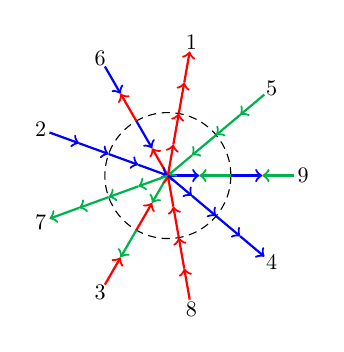
\begin{tikzpicture}[scale=.4,every node/.style={scale=.8}]

	%% Settings
	\pgfmathsetmacro{\Nutzahl}{9}

	\pgfmathsetmacro{\winkel}{360/\Nutzahl}

	\tikzstyle{outside}=[->, thick]
	\tikzstyle{inside}=[<-, thick]
	
	\draw[densely dashed] (0,0) circle (2);
	
	\foreach \i in {1,2,...,\Nutzahl}
	{	
		\node at (2*\i*\winkel:4.3) {\i};		
	}

	\begin{scope} [rotate=(0)*\winkel]
		\draw [color=blue, outside] (0:0) -- (0:1);
		\draw [color=green!70!blue, inside] (0:1) -- (0:2);
		\draw [color=blue, outside] (0:2) -- (0:3);
		\draw [color=green!70!blue, inside] (0:3) -- (0:4);
	\end{scope}

	\begin{scope} [rotate=(1)*\winkel]
		\draw [color=green!70!blue, inside] (0:0) -- (0:1);
		\draw [color=green!70!blue, inside] (0:1) -- (0:2);
		\draw [color=green!70!blue, inside] (0:2) -- (0:3);
		\draw [color=green!70!blue, inside] (0:3) -- (0:4);
	\end{scope}

	\begin{scope} [rotate=(2)*\winkel]
		\draw [color=red, outside] (0:0) -- (0:1);
		\draw [color=red, outside] (0:1) -- (0:2);
		\draw [color=red, outside] (0:2) -- (0:3);
		\draw [color=red, outside] (0:3) -- (0:4);
	\end{scope}

	\begin{scope} [rotate=(3)*\winkel]
		\draw [color=red, outside] (0:0) -- (0:1);
		\draw [color=blue, inside] (0:1) -- (0:2);
		\draw [color=red, outside] (0:2) -- (0:3);
		\draw [color=blue, inside] (0:3) -- (0:4);
	\end{scope}

	\begin{scope} [rotate=(4)*\winkel]
		\draw [color=blue, inside] (0:0) -- (0:1);
		\draw [color=blue, inside] (0:1) -- (0:2);
		\draw [color=blue, inside] (0:2) -- (0:3);
		\draw [color=blue, inside] (0:3) -- (0:4);
	\end{scope}

	\begin{scope} [rotate=(5)*\winkel]
		\draw [color=green!70!blue, outside] (0:0) -- (0:1);
		\draw [color=green!70!blue, outside] (0:1) -- (0:2);
		\draw [color=green!70!blue, outside] (0:2) -- (0:3);
		\draw [color=green!70!blue, outside] (0:3) -- (0:4);
	\end{scope}

	\begin{scope} [rotate=(6)*\winkel]
		\draw [color=green!70!blue, outside] (0:0) -- (0:1);
		\draw [color=red, inside] (0:1) -- (0:2);
		\draw [color=green!70!blue, outside] (0:2) -- (0:3);
		\draw [color=red, inside] (0:3) -- (0:4);
	\end{scope}

	\begin{scope} [rotate=(7)*\winkel]
		\draw [color=red, inside] (0:0) -- (0:1);
		\draw [color=red, inside] (0:1) -- (0:2);
		\draw [color=red, inside] (0:2) -- (0:3);
		\draw [color=red, inside] (0:3) -- (0:4);
	\end{scope}

	\begin{scope} [rotate=(8)*\winkel]
		\draw [color=blue, outside] (0:0) -- (0:1);
		\draw [color=blue, outside] (0:1) -- (0:2);
		\draw [color=blue, outside] (0:2) -- (0:3);
		\draw [color=blue, outside] (0:3) -- (0:4);
	\end{scope}

\end{tikzpicture}
%!tikz source end

    \end{center}
\end{minipage}
\begin{minipage}{.5\columnwidth}
    \begin{center}
        %!tikz editor 1.0
%!tikz source begin
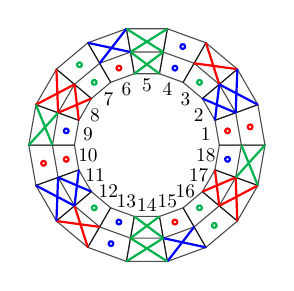
\begin{tikzpicture}[scale=.4,every node/.style={scale=.7}]

	%% Settings
	\pgfmathsetmacro{\Nutzahl}{18}
	\pgfmathsetmacro{\Spulenweite}{2}	

	\pgfmathsetmacro{\rNummerInnen}{1.9}
	\pgfmathsetmacro{\rInnen}{2.3}
	\pgfmathsetmacro{\rMitte}{3}
	\pgfmathsetmacro{\rAussen}{3.75}
	\pgfmathsetmacro{\rAngleOffset}{360/\Nutzahl/2}
	
	%% Background Pattern
	\foreach \i in {1,2,...,\Nutzahl}
	{	
		\draw [opacity=0.7] [rotate=(\i-1)*(360/\Nutzahl)]
			(0:\rMitte) -- (0:\rAussen) -- (360/\Nutzahl:\rAussen) -- (360/\Nutzahl:\rMitte) -- (0:\rMitte)
			(0:\rInnen) -- (0:\rMitte) -- (360/\Nutzahl:\rMitte) -- (360/\Nutzahl:\rInnen) -- (0:\rInnen);
		\node at (\i*360/\Nutzahl-\rAngleOffset:\rNummerInnen) {\i};		
	}

	%% Inner
	% red
	\foreach \i in {1,6,10,15}
	{	
		\draw [rotate=(\i-1)*(360/\Nutzahl), thick, color=red]
			(180/\Nutzahl:2.6) circle (0.075);
		\draw [rotate=(\i-1+\Spulenweite)*(360/\Nutzahl), thick, color=red]
			(0:\rMitte) -- (360/\Nutzahl:\rAussen) (0:\rAussen) -- (360/\Nutzahl:\rMitte);
	}
	\foreach \i in {8,17}
	{	
		\draw [rotate=(\i-1)*(360/\Nutzahl), thick, color=red]
			(0:\rInnen) -- (360/\Nutzahl:\rMitte) (0:\rMitte) -- (360/\Nutzahl:\rInnen);
		\draw [rotate=(\i-1+\Spulenweite)*(360/\Nutzahl), thick, color=red]
			(180/\Nutzahl:3.33) circle (0.075);
	}
	
	% blue
	\foreach \i in {4,9,13,18}
	{	
		\draw [rotate=(\i-1)*(360/\Nutzahl), thick, color=blue]
			(180/\Nutzahl:2.6) circle (0.075);
		\draw [rotate=(\i-1+\Spulenweite)*(360/\Nutzahl), thick, color=blue]
			(0:\rMitte) -- (360/\Nutzahl:\rAussen) (0:\rAussen) -- (360/\Nutzahl:\rMitte);
	}
	\foreach \i in {2,11}
	{	
		\draw [rotate=(\i-1)*(360/\Nutzahl), thick, color=blue]
			(0:\rInnen) -- (360/\Nutzahl:\rMitte) (0:\rMitte) -- (360/\Nutzahl:\rInnen);
		\draw [rotate=(\i-1+\Spulenweite)*(360/\Nutzahl), thick, color=blue]
			(180/\Nutzahl:3.33) circle (0.075);
	}
	
	% green
	\foreach \i in {3,7,12,16}
	{	
		\draw [rotate=(\i-1)*(360/\Nutzahl), thick, color=green!70!blue]
			(180/\Nutzahl:2.6) circle (0.075);
		\draw [rotate=(\i-1+\Spulenweite)*(360/\Nutzahl), thick, color=green!70!blue]
			(0:\rMitte) -- (360/\Nutzahl:\rAussen) (0:\rAussen) -- (360/\Nutzahl:\rMitte);
	}
	\foreach \i in {5,14}
	{	
		\draw [rotate=(\i-1)*(360/\Nutzahl), thick, color=green!70!blue]
			(0:\rInnen) -- (360/\Nutzahl:\rMitte) (0:\rMitte) -- (360/\Nutzahl:\rInnen);
		\draw [rotate=(\i-1+\Spulenweite)*(360/\Nutzahl), thick, color=green!70!blue]
			(180/\Nutzahl:3.33) circle (0.075);
	}
	
\end{tikzpicture}
%!tikz source end

    \end{center}
\end{minipage}

}
